
The objective of ancillary services can generally be defined as: maintaining an adequate and secure power system. This means maintaining the power system operating at nominal frequency and voltage. In cases where the power system deviates from nominal operation, either due to natural fluctuations in consumption or faults in the system, the system operators will activate ancillary services to restore normal operation.


%%%%%%%%%%%%%%%%%%%%%%%
\subsection{The function of ancillary services}
%%%%%%%%%%%%%%%%%%%%%%%
%\textcolor{red}{We want to describe what is the purpose of the AS that are within scope, and describe which physical need they are covering}

In the electricity system, supply and demand must be kept balanced at all times and two metrics are commonly used to evaluate the current imbalance in a power system: system frequency and the area control error (ACE). System frequency is a measure of the speed at which all interconnected, synchronous generators are rotating.  ACE is a measure of the deviation in scheduled power exchanges between interconnected electricity systems. 

System imbalances have two causes:
\begin{enumerate}
\item Expected imbalances due to deviations between the planned generation and the actual electricity demand.
\item Unexpected imbalances due to system contingency.
\end{enumerate}

System operators procure ancillary services\footnote{Ancillary services are also used to solve other operating issues in the power system, such as voltage problems, but this work will focus specifically on frequency services.} in order to deal with these imbalances in their daily operation. The structure of the ancillary services varies between systems but can generally be divided into primary, secondary and tertiary control\footnote{Recently, ENTSO-E has changed its terminology for AS providing Load-Frequency Control to Frequency Containment Reserves, Frequency Restoration Reserves (either automatic or manual), and Replacement Reserves\cite{entsoe2013network}. This classification matches roughly into the framework presented in \cite{Rebours}.}\cite{Rebours}. This work will focus specifically on the primary and secondary frequency control.

\subsection*{Primary Frequency Control}
Primary frequency control is the fastest response (in the seconds range) and is used to arrest and begin reversing frequency excursions occurring due to sudden imbalances between supply and demand, often caused by contingency events. Primary frequency control is traditionally performed by generators under ``droop'' control, in which a  change in power output is made proportional to locally measured frequency. The reason for this is that the response to the frequency excursion must occur as fast as possible and be proportional to the size of the excursion so that the system frequency stabilizes within an acceptable time frame.
\subsection*{Secondary Frequency Control}
Secondary frequency control is a slower response (in the seconds to minute range) that takes over for the primary frequency control and returns the system to nominal frequency by controlling the output of participating resources. Much more urgently, it restores the full bipolar range of the primary reserve, so the system gets back to nominal $n-1$ redundancy. Usually an entity estimates the control reference signals based upon the ACE and system frequency to simultaneously resolve the imbalance at the interconnection and maintain stable operation (see, e.g. \cite{nerc2011balancing,entsoe2014continental}, for more details). The control algorithm that directly controls the output of resources providing this service is often called Automatic Generation Control (AGC)\footnote{This balancing control logic can have a centralized, pluralistic or hierarchical architecture~\cite{entsoe2014continental} to determine the individual reference signals for the generators.}. The generators will have either a proportional controller or a proportional-integral (PI) controller to track the AGC signal. The secondary response also needs to occur as fast as possible, yet due to its centralised control approach, it is not able to provide as fast a response as primary control. The underlying need for the secondary service is to supply a fast reference tracking response without overshoot.



\subsection*{Addressing the need}
%\olge{This section duplicates quite a lot of information from the previous one. Maybe they could be joined?}
An illustration of the power system frequency during a contingency is shown in Fig.~\ref{fig:contingency}. When a system contingency occurs, such as the loss of a large generator or a transmission line, there is a sudden loss in generation that is made up for by the small amount of inherent storage in the rotating inertia of the remaining synchronous generators. This sudden loss reduces the rotational speed of said generators which results in a frequency excursion whose slope is determined by the total inertia of the system. The inertia of the system is determined by the amount of kinetic energy in the synchronous generators in the system, and as these generators are decommissioned, the inertia in the system will decrease, thus increasing the volatility of the system. Until now, system operators have been able to arrest frequency excursions fast enough because of the inherent system inertia, but as the inertia decreases, faster response times are required of the primary frequency control. 

The system operator must have enough primary reserves to arrest the frequency as fast as possible, before the system enters a state where a blackout is inevitable. A metric for how effective the procurement of reserve is the \emph{frequency nadir} \cite{eto2010use}, and it is desirable that the value is as close as possible to the nominal frequency of the system.

Similarly, the system operator should ensure that the secondary reserves act as fast as possible to relieve the primary reserves and also bring the frequency from the settling frequency back to the nominal frequency.

In \cite{vrettos2015integrating} it is shown that if primary frequency response is provided by demand response (with a very fast response), the frequency nadir occurs at higher frequencies. 
Also, in \cite{makarov2008assessing}, the authors argue that the value of regulation resources can be defined based upon the ramp capabilities of the service providing units. Faster reacting units are more valuable to system operators, since they help arrest the frequency excursion faster and at a higher nadir. It does require changes to the AGC in order to utilize the fast response, but this would also lead to the need for fewer reserves.

\begin{figure}[htbp!]
\centering
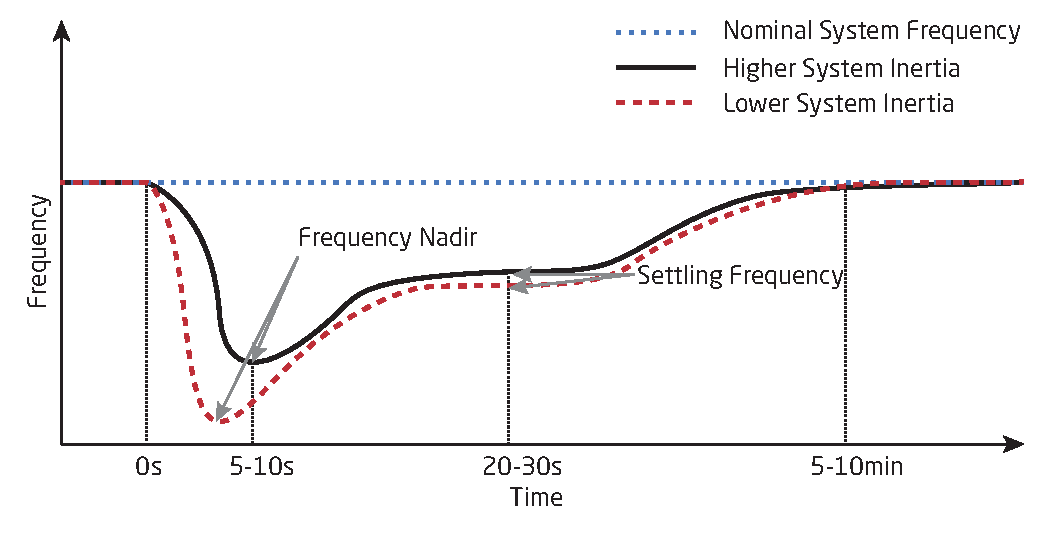
\includegraphics[width=1\columnwidth]{frequency_contingency.eps}
\caption{The nadir of a system frequency excursion during contingency events is more pronounced if there is less inertia in the system.}
\label{fig:contingency}
\end{figure}

%%%%%%%%%%%%%%%%%%%%%%%
\subsection{Ancillary service procurement and service  requirements}\label{sec:procurement}
%%%%%%%%%%%%%%%%%%%%%%
%\textcolor{red}{we talked about the needs, they are tackled by the following requirements, due to historical, computational reasons. Here it should be made clear in which way the current requirements do not exploit the full capabilities of all units}

\subsection*{Procurement requirements}
All electrical power systems require ancillary services, but not all system operators acquire them through market mechanisms. In the US, primary frequency control is expected to be part of the normal operation of the generators, and is therefore not directly compensated. In other cases, AS are bundled within bilateral energy contracts as one product contracted by the system operator.

In all instances, the system operators have procurement requirements that are dimensioned through static analysis of the system. Until recently, measurement equipment has not been able to measure the frequency nadir\cite{eto2010use}. Consequently, the dimensioning of the primary reserves has been made on the settling frequency, parting from static offline calculations of the dynamics of the grid. Typically, system operators are required to contract reserves corresponding to a percentage of the overall system load, e.g. regulation reserves usually cover 1\% of the load, or cover the loss of specific units, e.g. the \emph{N-1} criteria.


\subsection*{Service Requirements}
Because AS are essential for the secure operation of the system, the system operators also have requirements and restrictions on the units providing AS. A super-set of requirements across different systems is defined in \cite{Rebours}. These requirements can roughly be classified into three categories: \emph{temporal requirements}, which relate to how fast and for how long a service must be delivered; \emph{resource tuning requirements}, which relate to specific values that tuning parameters in the resource must have; and \emph{market requirements}, which relate to bid sizes and similar parameters in systems where services are acquired through market mechanisms. Of these three categories, only the temporal requirements relate to service performance. Furthermore, in most systems are the requirements implicitly defined for traditional generation units. This means that most service requirements are oriented towards the least common denominator of service providers, e.g. a unit providing primary frequency control should provide half of the service within 15 seconds and full response within 30 seconds\cite{energinet2012ancillary}. A variety of generation and consumption units would be able to provide this service faster, but this quality is not rewarded. Another example is the requirement of having a PI-controller on units providing secondary frequency control, in order to track the AGC signal. Such a controller is infeasible on distributed systems, but other modern controllers can provide offset-free control with similar properties.


%Units which do not perform within the specified requirements are heavily fined. \macd{I assume there will be more to follow this statement?}\bondy{Yeah, I had hoped you might want to write a line or two here :-).}
%\textcolor{red}{Joe wants us to go much more in depth on this point, for example discuss how PJM has reg A and D}
%
\subsection*{Impacts of historical requirements}

%\bondy{(The following section should make it clear why the new resources would be utilized suboptimally if they have to comply to current requirements. I'm having problems tackling this section, perhaps Kai and Jason could help?, also, the title of the section should perhaps be changed?)} \macd{Perhaps the title of this section should be "Impacts of historical requirements", or something like that. }

In short, the historical definitions for service requirements results in the suboptimal use of today's AS resources. Due to the legacy definitions there is an implicit %explicit 
bias for traditional resources, and alternative technologies, such as demand response, are are restricted in their contribution to AS provision, and their favorable properties are not utilized or undervalued.

While system operators have been able to maintain a secure system using traditional resources, the changes in the power system, i.e. the decrease of system inertia and increased fluctuation due to RES, require units that react faster than the current minimum requirements. Also, an increased overall volume of balancing resources will be required due to the larger deviations caused by the RES.
Units that provide a faster response but are not able to provide the full response duration should be enabled to contribute to AS provision and be valued accordingly.

If these technologies, both the underutilized and the ones restricted from providing services, are used optimally for ancillary service delivery, it follows from the conclusions presented in \cite{makarov2008assessing,vrettos2015integrating} that frequency excursions could be arrested at higher frequency nadir, thus lessening the required amount of reserves, which leads to a lower-cost operation of the system. 
Regulative authorities have concluded that fast reacting units are valuable for the system operation, and started programs to benefit of these resources. An example of this is FERC order 755 (Pay for Performance) which has led to PJM splitting their regulation market product into RegA, for slow reacting units, and RegD for fast reacting units. The product differentiation approach has been a success for PJM, but splitting the market into different products does not address two points: 1) the overall pool of resources will not be optimally utilized, and 2) as other new technologies appear in the system, the market might fragment further, also leading to non-optimal utilization of resources.  We propose instead to restructure the ancillary service definitions such that all types of service providers participate with the same market product defined by a set of optimal performance parameters, and not by minimum requirements. This means that the all entities providing a given ancillary service, e.g. primary frequency control, are optimally cleared under a single market. The service restructuring is detailed in the following section.
